\documentclass[12pt]{article}\usepackage[]{graphicx}\usepackage[]{color}
%% maxwidth is the original width if it is less than linewidth
%% otherwise use linewidth (to make sure the graphics do not exceed the margin)
\makeatletter
\def\maxwidth{ %
  \ifdim\Gin@nat@width>\linewidth
    \linewidth
  \else
    \Gin@nat@width
  \fi
}
\makeatother

\definecolor{fgcolor}{rgb}{0.345, 0.345, 0.345}
\newcommand{\hlnum}[1]{\textcolor[rgb]{0.686,0.059,0.569}{#1}}%
\newcommand{\hlstr}[1]{\textcolor[rgb]{0.192,0.494,0.8}{#1}}%
\newcommand{\hlcom}[1]{\textcolor[rgb]{0.678,0.584,0.686}{\textit{#1}}}%
\newcommand{\hlopt}[1]{\textcolor[rgb]{0,0,0}{#1}}%
\newcommand{\hlstd}[1]{\textcolor[rgb]{0.345,0.345,0.345}{#1}}%
\newcommand{\hlkwa}[1]{\textcolor[rgb]{0.161,0.373,0.58}{\textbf{#1}}}%
\newcommand{\hlkwb}[1]{\textcolor[rgb]{0.69,0.353,0.396}{#1}}%
\newcommand{\hlkwc}[1]{\textcolor[rgb]{0.333,0.667,0.333}{#1}}%
\newcommand{\hlkwd}[1]{\textcolor[rgb]{0.737,0.353,0.396}{\textbf{#1}}}%
\let\hlipl\hlkwb

\usepackage{framed}
\makeatletter
\newenvironment{kframe}{%
 \def\at@end@of@kframe{}%
 \ifinner\ifhmode%
  \def\at@end@of@kframe{\end{minipage}}%
  \begin{minipage}{\columnwidth}%
 \fi\fi%
 \def\FrameCommand##1{\hskip\@totalleftmargin \hskip-\fboxsep
 \colorbox{shadecolor}{##1}\hskip-\fboxsep
     % There is no \\@totalrightmargin, so:
     \hskip-\linewidth \hskip-\@totalleftmargin \hskip\columnwidth}%
 \MakeFramed {\advance\hsize-\width
   \@totalleftmargin\z@ \linewidth\hsize
   \@setminipage}}%
 {\par\unskip\endMakeFramed%
 \at@end@of@kframe}
\makeatother

\definecolor{shadecolor}{rgb}{.97, .97, .97}
\definecolor{messagecolor}{rgb}{0, 0, 0}
\definecolor{warningcolor}{rgb}{1, 0, 1}
\definecolor{errorcolor}{rgb}{1, 0, 0}
\newenvironment{knitrout}{}{} % an empty environment to be redefined in TeX

\usepackage{alltt}
\usepackage{scrtime} % for \thistime (this package MUST be listed first!)
\usepackage[margin=1in]{geometry}
\usepackage{subfig}

%% Language and font encodings
\usepackage[english]{babel}
\usepackage[utf8x]{inputenc}
\usepackage[T1]{fontenc}

%% Useful packages
\usepackage{amsmath}
\usepackage{amsthm} % for theorems and proofs
\usepackage{amsfonts} % mathbb
\usepackage{graphicx}
\usepackage[colorinlistoftodos]{todonotes}
\definecolor{aqua}{RGB}{0, 128, 225}
\usepackage[colorlinks=true,citecolor=aqua,linkcolor=aqua,urlcolor=aqua]{hyperref}
\usepackage[nameinlink]{cleveref}
\usepackage{lineno}

\usepackage{fancyhdr,lastpage}
\pagestyle{fancy}
\fancyhf{} % clear all header and footer parameters
%%%\lhead{Student Name: \theblank{4cm}}
%%%\chead{}
%%%\rhead{Student Number: \theblank{3cm}}
%%%\lfoot{\small\bfseries\ifnum\thepage<\pageref{LastPage}{CONTINUED\\on next page}\else{LAST PAGE}\fi}
\lfoot{}
\cfoot{{\small\bfseries Page \thepage\ of \pageref{LastPage}}}
\rfoot{}
\renewcommand\headrulewidth{0pt} % Removes funny header line

\newcommand{\R}{{\cal R}}

\title{Synchrony and Persistence of Recurrent Epidemics (Supplementary Material)}
\author{\underline{\emph{Group Name}}: \texttt{{\color{blue}The Infective Collective}}\\
{}\\
\underline{\emph{Group Members}}: {\color{blue}Aurora Basinski-Ferris, Michael Chong, Daniel Park, Daniel Presta}}

\date{\today\ @ \thistime}
\IfFileExists{upquote.sty}{\usepackage{upquote}}{}
\begin{document}


\linenumbers
\maketitle

\section{Introduction}
This supplement contains the necessary code to reproduce the data and graphs in the main paper. We also include additional discussion and explanation of some of our methods and results.

\section{The Model}

\subsection{Construction of the model}

Here, we provide a detailed derivation of the model.
First, consider the following coupled SIR model consisting of $n$ patches:
\begin{equation}
\begin{aligned}
\frac{dS_k}{dt} &= \mu N - \left(\sum_{j=1}^n \beta(t) m_{kj} I_j + \mu\right) S_k \\
\frac{dI_k}{dt} &= \left(\sum_{j=1}^n \beta(t) m_{kj} I_j + \mu\right) S_k - (\mu  + \gamma) I_k\\
\frac{dR_k}{dt} &= \gamma I_k - \mu R_k
\end{aligned}
\end{equation}
where $S_k$, $I_k$ and $R_k$ are numbers of susceptible, infected and recovered individuals in patch $k$, respectively. 
$N$ is population size in every patch and is assumed to be constant. 
$\beta(t)$ is the transmission rate, $\gamma$ is the per capita recovery rate and $\mu$ is the per capita death rate as well as birth rate. 
$m_{kj}$ is the proportion of contacts from patch $j$ that are dispersed to patch $k$. 
The dispersal matrix is then given by $M = \left[m_{kj}\right]$ and we have $\sum_{k=1}^n m_{kj} = 1$. 

Note that a susceptible individual in patch $i$ leaves the susceptible compartment at rate $\sum_{j=1}^n \beta(t) m_{ij} I_j + \mu$. We can view this quantity as hazard and obtain the probability that a susceptible individual survives during a time interval $(t, t + \Delta t)$:
\begin{equation}
\exp \left(-\int_{t}^{t + \Delta t} \sum_{j=1}^n \beta(s) m_{kj} I_j(s) + \mu d s \right),
\end{equation}
where for sufficiently small $\Delta t$, we can write
\begin{equation}
\int_{t}^{t + \Delta t} \sum_{j=1}^n \beta(s) m_{kj} I_j(s) + \mu d s \approx \left(\sum_{j=1}^n \beta(t) m_{kj} I_j(s) + \mu \right) \Delta t.
\end{equation}
Rearranging, number of individuals that leave the susceptible compartment after $\Delta$ time step is given by
\begin{equation}
S_{k, \tiny{\textrm{leave}}}(t) = \left(1 - \exp \left(-\left(\sum_{j=1}^n \beta(t) m_{kj} I_j(s) + \mu \right) \Delta t \right) \right) S_k(t)
\end{equation}
Assuming that the transmission rate and number of infected individuals stays constant over the interval $(t, t+\Delta)$, the probability that a susceptible individual leaves the compartment due to infection is given by 
\begin{equation}
\frac{\sum_{j=1}^n \beta(t) m_{kj} I_j(s)}{\sum_{j=1}^n \beta(t) m_{kj} I_j(s) + \mu}
\end{equation}
Incidence (i.e., number of suseptible individuals that become infected during $(t, t+\Delta t)$ interval) is then given by the product of above probability and $S_{i, \tiny{\textrm{leave}}}(t)$.
Similarly, an infected individual and a recovered individual suffer from constant hazard of $\gamma + \mu$ and $\mu$, respectively.
Since these rates are not time-dependent, these can each be translated into transition probabilities assuming exponentially distributed life time in each compartment, yielding
\begin{equation}
\begin{aligned}
I_{k, \tiny{\textrm{leave}}}(t) &= (1 - \exp(-(\gamma + \mu)\Delta t)) I_k(t) \\
R_{k, \tiny{\textrm{leave}}}(t) &= (1 - \exp(-\mu \Delta t)) R_k(t)
\end{aligned}
\end{equation}
Then, the full discrete time model is given by
\begin{equation}
\label{eq:discretedeterministic}
\begin{aligned}
S_{k}(t+\Delta t) &= b_k(t) + S_k(t) - S_{k, \tiny{\textrm{leave}}}(t)\\
I_{k}(t+\Delta t) &= i_k(t) + I_k(t) - I_{k, \tiny{\textrm{leave}}}(t)\\
R_{k}(t+\Delta t) &= r_k(t) + R_k(t) - R_{k, \tiny{\textrm{leave}}}(t)
\end{aligned}
\end{equation}
where $b_k(t)$, $i_k(t)$, and $r_k(t)$ represent number of new susceptible, infected, and recovered individuals that are produced between the interval $(t, t+\Delta t)$:
\begin{equation}
\begin{aligned}
i_k(t) &= \frac{\sum_{j=1}^n \beta(t) m_{ij} I_j(s)}{\sum_{j=1}^n \beta(t) m_{ij} I_j(s) + \mu} S_{k, \tiny{\textrm{leave}}}(t)\\
r_k(t) &= \frac{\gamma}{\gamma + \mu} R_{k, \tiny{\textrm{leave}}}(t)\\
b_k(t) &= S_{k, \tiny{\textrm{leave}}}(t) - i_k(t) + I_{k, \tiny{\textrm{leave}}}(t) - r_k(t)\\
\end{aligned}
\end{equation}

\subsection{Time-dependent transmission rate}

Since many recurrent epidemics are childhood diseases, we choose to look at a time-dependent transmission rate that is dependent on an elementary student's school year. From Bauch and Earn, we define the time-dependent transmission rate as

\begin{equation}
\begin{aligned}
\beta (t) &=
\begin{cases} b_0 (1 + 2(1 - p_s) b_1) &\mbox{school days} \\
b_0 (1 - 2 p_s b_1) & \mbox{non-school days}
\end{cases},
\end{aligned}
\end{equation}
where $b_0$ is the mean transmission rate, $b_1 = =0.25$ is the amplitude of the term-time forcing, and $p_s = 0.7589$ is the approximate proportion of the year that falls in the school term. We define our school days and non-school days in the following manner (all dates inclusive, leap years not considered):

\begin{itemize}
\item Each day (including weekends) from January 7th to March 9th is considered a school day.
\item Each day from March 10th to March 17th is a non-school day, since March break approximately occurs during this time of year.
\item Each day (including weekends) from March 18th to June 30th is a school day.
\item Each day from July 1st to September 3rd is a non-school day, as summer vacation occurs during this time.
\item Each day from September 4th to December 22nd is a school day.
\item Each day from December 23rd to January 6th is a non-school day (Christmas, New Years break).
\end{itemize}

We chose these days after examining past school calendars from the Toronto District School Board and making reasonable assumptions regarding the average school opening and school closing dates, as well as the average beginning and end dates of school breaks. Furthermore, we included weekends to account for contact-heavy children's extracurricular activities that may take place on weekends during the school year, and to make the code easier to implement (greatly reduce the number of ``\texttt{if}" statements).

\subsection{Load packages}

Before we attempt any numerical analysis, we want to load all necessary pacakges first.

\begin{knitrout}
\definecolor{shadecolor}{rgb}{0.969, 0.969, 0.969}\color{fgcolor}\begin{kframe}
\begin{alltt}
\hlkwd{library}\hlstd{(Rcpp)}
\hlkwd{library}\hlstd{(deSolve)}
\hlkwd{library}\hlstd{(tidyr)}
\hlkwd{library}\hlstd{(dplyr)}
\hlkwd{library}\hlstd{(ggplot2);} \hlkwd{theme_set}\hlstd{(}\hlkwd{theme_bw}\hlstd{(}\hlkwc{base_size} \hlstd{=} \hlnum{12}\hlstd{,}
                                     \hlkwc{base_family} \hlstd{=} \hlstr{"Times"}\hlstd{))}
\hlkwd{library}\hlstd{(gridExtra)}
\hlkwd{library}\hlstd{(stringr)}

\hlkwa{if} \hlstd{(.Platform}\hlopt{$}\hlstd{OS.type}\hlopt{==}\hlstr{"windows"}\hlstd{) \{}
    \hlkwd{windowsFonts}\hlstd{(}\hlkwc{Times}\hlstd{=}\hlkwd{windowsFont}\hlstd{(}\hlstr{"Times"}\hlstd{))}
\hlstd{\}}
\end{alltt}
\end{kframe}
\end{knitrout}

\subsection{Implementation of the model}

Implementation of the model is done using the \texttt{Rcpp} package.
The source code is too long to be displayed here. 
Interested readers should look at the source code \texttt{SIRmodel\_npatch.cpp}.
Before we perform any analysis, we have to load the model file:
\begin{knitrout}
\definecolor{shadecolor}{rgb}{0.969, 0.969, 0.969}\color{fgcolor}\begin{kframe}
\begin{alltt}
\hlkwd{sourceCpp}\hlstd{(}\hlstr{"SIRmodel_npatch.cpp"}\hlstd{)}
\end{alltt}


{\ttfamily\noindent\color{warningcolor}{\#\# Warning in normalizePath(file, winslash = "{}/"{}): path[1]="{}SIRmodel\_npatch.cpp"{}: No such file or directory}}

{\ttfamily\noindent\bfseries\color{errorcolor}{\#\# Error in sourceCpp("{}SIRmodel\_npatch.cpp"{}): file not found: 'SIRmodel\_npatch.cpp'}}\end{kframe}
\end{knitrout}

\subsection{Parameters}

Base parameters are stored as a list.

\begin{knitrout}
\definecolor{shadecolor}{rgb}{0.969, 0.969, 0.969}\color{fgcolor}\begin{kframe}
\begin{alltt}
\hlstd{base.params} \hlkwb{<-} \hlkwd{list}\hlstd{(}
    \hlkwc{R0}\hlstd{=}\hlnum{17}\hlstd{,}
    \hlkwc{pop}\hlstd{=}\hlnum{1e6}\hlstd{,}
    \hlkwc{b1}\hlstd{=}\hlnum{0.25}\hlstd{,}
    \hlkwc{gamma}\hlstd{=}\hlnum{365}\hlopt{/}\hlnum{13}\hlstd{,}
    \hlkwc{mu}\hlstd{=}\hlnum{0.02}\hlstd{,}
    \hlkwc{dt}\hlstd{=}\hlnum{1}\hlopt{/}\hlnum{365}\hlstd{,}
    \hlkwc{nsteps}\hlstd{=}\hlnum{365}\hlopt{*}\hlnum{100}
\hlstd{)}
\end{alltt}
\end{kframe}
\end{knitrout}


Here, we deinfe a function named \texttt{initfun} that returns states at the endemic equilibrium assuming constant transmission rate.

\begin{knitrout}
\definecolor{shadecolor}{rgb}{0.969, 0.969, 0.969}\color{fgcolor}\begin{kframe}
\begin{alltt}
\hlstd{initfun} \hlkwb{<-} \hlkwa{function}\hlstd{(}\hlkwc{param}\hlstd{,}
                    \hlkwc{n.patch}\hlstd{=}\hlnum{1}\hlstd{,}
                    \hlkwc{round}\hlstd{=}\hlnum{FALSE}\hlstd{) \{}
    \hlkwd{with}\hlstd{(param,\{}
        \hlstd{epsilon} \hlkwb{<-} \hlstd{mu}\hlopt{/}\hlstd{(mu}\hlopt{+}\hlstd{gamma)}

        \hlstd{ll} \hlkwb{<-} \hlkwd{list}\hlstd{(}
            \hlkwc{S}\hlstd{=}\hlkwd{rep}\hlstd{(pop}\hlopt{/}\hlstd{R0, n.patch),}
            \hlkwc{I}\hlstd{=}\hlkwd{rep}\hlstd{(epsilon}\hlopt{*}\hlstd{(}\hlnum{1}\hlopt{-}\hlnum{1}\hlopt{/}\hlstd{R0)}\hlopt{*}\hlstd{pop, n.patch)}
        \hlstd{)}

        \hlkwa{if} \hlstd{(round) ll} \hlkwb{<-} \hlkwd{lapply}\hlstd{(ll, round)}

        \hlstd{ll}\hlopt{$}\hlstd{R} \hlkwb{<-} \hlstd{pop} \hlopt{-} \hlstd{ll}\hlopt{$}\hlstd{S} \hlopt{-} \hlstd{ll}\hlopt{$}\hlstd{I}

        \hlstd{ll}
    \hlstd{\})}
\hlstd{\}}
\end{alltt}
\end{kframe}
\end{knitrout}

Base initial conditions are then equal to endemic equilibrium.

\begin{knitrout}
\definecolor{shadecolor}{rgb}{0.969, 0.969, 0.969}\color{fgcolor}\begin{kframe}
\begin{alltt}
\hlstd{base.init} \hlkwb{<-} \hlkwd{initfun}\hlstd{(base.params)}
\end{alltt}
\end{kframe}
\end{knitrout}

\section{Bifurcation diagram}

In order to make a bifurcation diagram, we vary $\R_0$ from 1 to 20 every 0.2 steps. 
Then, for each $\R_0$, 20 simulations are run from random initial conditions for 4000 years to remove any transient behaviours that might be present.
Here, we check whether the simulation file is present. If not, simulations are run and saved as an \texttt{.rda} file.
Note that this simulation takes approximately 20 hours. Thus, we load a saved file instead.

\begin{knitrout}
\definecolor{shadecolor}{rgb}{0.969, 0.969, 0.969}\color{fgcolor}\begin{kframe}
\begin{alltt}
\hlkwa{if} \hlstd{(}\hlkwd{file.exists}\hlstd{(}\hlstr{"bifurcation.rda"}\hlstd{)) \{}
    \hlkwd{load}\hlstd{(}\hlstr{"bifurcation.rda"}\hlstd{)}
\hlstd{\}} \hlkwa{else} \hlstd{\{}
    \hlstd{nsim} \hlkwb{<-} \hlnum{20}
    \hlstd{R0vec} \hlkwb{<-} \hlkwd{seq}\hlstd{(}\hlnum{1}\hlstd{,} \hlnum{20}\hlstd{,} \hlkwc{by}\hlstd{=}\hlnum{0.2}\hlstd{)}

    \hlkwd{set.seed}\hlstd{(}\hlnum{101}\hlstd{)}
    \hlstd{init} \hlkwb{<-} \hlkwd{data.frame}\hlstd{(}
        \hlkwc{S}\hlstd{=}\hlkwd{seq}\hlstd{(}\hlkwc{from}\hlstd{=}\hlnum{0}\hlstd{,} \hlkwc{to}\hlstd{=}\hlnum{0.1}\hlstd{,} \hlkwc{length.out}\hlstd{=nsim)} \hlopt{*} \hlstd{base.params[[}\hlstr{"pop"}\hlstd{]],}
        \hlkwc{I}\hlstd{=}\hlkwd{seq}\hlstd{(}\hlkwc{from}\hlstd{=}\hlnum{0}\hlstd{,} \hlkwc{to}\hlstd{=}\hlnum{0.0001}\hlstd{,} \hlkwc{length.out}\hlstd{=nsim)} \hlopt{*} \hlstd{base.params[[}\hlstr{"pop"}\hlstd{]]}
    \hlstd{)}

    \hlstd{init[]} \hlkwb{<-} \hlkwd{apply}\hlstd{(init,} \hlnum{2}\hlstd{, sample)}
    \hlstd{init}\hlopt{$}\hlstd{R} \hlkwb{<-} \hlstd{base.params[[}\hlstr{"pop"}\hlstd{]]} \hlopt{-} \hlstd{(init}\hlopt{$}\hlstd{S} \hlopt{+} \hlstd{init}\hlopt{$}\hlstd{I)}

    \hlstd{blist} \hlkwb{<-} \hlkwd{vector}\hlstd{(}\hlstr{'list'}\hlstd{,} \hlkwd{length}\hlstd{(R0vec))}

    \hlkwa{for} \hlstd{(R} \hlkwa{in} \hlstd{R0vec) \{}

        \hlstd{pp} \hlkwb{<-} \hlstd{base.params}
        \hlstd{pp[[}\hlstr{"R0"}\hlstd{]]} \hlkwb{<-} \hlstd{R}
        \hlstd{pp[[}\hlstr{"nsteps"}\hlstd{]]} \hlkwb{<-} \hlnum{365} \hlopt{*} \hlnum{4000}

        \hlstd{blist[[}\hlkwd{which}\hlstd{(R0vec}\hlopt{==}\hlstd{R)]]} \hlkwb{<-} \hlkwd{lapply}\hlstd{(}\hlnum{1}\hlopt{:}\hlstd{nsim,} \hlkwa{function}\hlstd{(}\hlkwc{x}\hlstd{)\{}
            \hlstd{ii} \hlkwb{<-} \hlstd{init[x,]}
            \hlstd{df} \hlkwb{<-} \hlkwd{SIRmodel_npatch}\hlstd{(pp, ii,} \hlkwd{matrix}\hlstd{(}\hlnum{1}\hlstd{), term_time)}
            \hlstd{prev} \hlkwb{<-} \hlkwd{tail}\hlstd{(df}\hlopt{$}\hlstd{I[df}\hlopt{$}\hlstd{time}\hlopt\hlnum{1}\hlopt{==}\hlnum{0}\hlstd{],} \hlnum{100}\hlstd{)}\hlopt{/}\hlstd{pp[[}\hlstr{"pop"}\hlstd{]]}

            \hlkwd{data.frame}\hlstd{(}
                \hlkwc{prevalence}\hlstd{=prev,}
                \hlkwc{R0}\hlstd{=R}
            \hlstd{)}
        \hlstd{\})}
            \hlkwd{save}\hlstd{(}\hlstr{"blist"}\hlstd{,} \hlkwc{file}\hlstd{=}\hlstr{"bifurcation.rda"}\hlstd{)}
        \hlstd{\}}

    \hlkwd{save}\hlstd{(}\hlstr{"blist"}\hlstd{,} \hlkwc{file}\hlstd{=}\hlstr{"bifurcation.rda"}\hlstd{)}

    \hlstd{\}}
\end{alltt}
\end{kframe}
\end{knitrout}

Once the simulation is done, we can clean the simulation data to generate a data frame that can be used to create a bifurcation diagram:

\begin{knitrout}
\definecolor{shadecolor}{rgb}{0.969, 0.969, 0.969}\color{fgcolor}\begin{kframe}
\begin{alltt}
\hlstd{bdf} \hlkwb{<-} \hlstd{blist} \hlopt
    \hlkwd{lapply}\hlstd{(bind_rows,} \hlkwc{.id}\hlstd{=}\hlstr{"sim"}\hlstd{)} \hlopt
    \hlstd{bind_rows}

\hlstd{bifur_df} \hlkwb{<-} \hlstd{bdf} \hlopt
    \hlkwd{group_by}\hlstd{(sim, R0)} \hlopt
    \hlkwd{filter}\hlstd{(prevalence} \hlopt{>} \hlnum{0}\hlstd{)} \hlopt
    \hlkwd{filter}\hlstd{(}\hlopt{!}\hlkwd{duplicated}\hlstd{(prevalence))} \hlopt
    \hlkwd{group_by}\hlstd{(R0)} \hlopt
    \hlkwd{filter}\hlstd{(}\hlopt{!}\hlkwd{duplicated}\hlstd{(}\hlkwd{round}\hlstd{(prevalence,} \hlnum{10}\hlstd{)))} \hlopt
    \hlkwd{group_by}\hlstd{(sim, R0)} \hlopt
    \hlkwd{mutate}\hlstd{(}
        \hlkwc{i}\hlstd{=}\hlkwd{n}\hlstd{()}
    \hlstd{)} \hlopt
    \hlkwd{group_by}\hlstd{(R0, i)} \hlopt
    \hlkwd{mutate}\hlstd{(}
        \hlkwc{prevalence}\hlstd{=}\hlkwd{ifelse}\hlstd{(i}\hlopt{==}\hlnum{1}\hlstd{,} \hlkwd{mean}\hlstd{(prevalence), prevalence)}
    \hlstd{)} \hlopt
    \hlkwd{filter}\hlstd{(}\hlopt{!}\hlkwd{duplicated}\hlstd{(prevalence))} \hlopt
    \hlkwd{group_by}\hlstd{()} \hlopt
    \hlkwd{mutate}\hlstd{(}
        \hlkwc{sim}\hlstd{=}\hlkwd{ifelse}\hlstd{(i}\hlopt{==}\hlnum{1}\hlstd{,} \hlnum{1}\hlstd{, sim)}
    \hlstd{)} \hlopt
    \hlkwd{group_by}\hlstd{(sim, R0, i)} \hlopt
    \hlkwd{mutate}\hlstd{(}
        \hlkwc{prevalence}\hlstd{=}\hlkwd{sort}\hlstd{(prevalence),}
        \hlkwc{j}\hlstd{=}\hlkwd{seq_along}\hlstd{(i)}
    \hlstd{)} \hlopt
    \hlstd{group_by} \hlopt
    \hlkwd{mutate}\hlstd{(}
        \hlkwc{sim}\hlstd{=}\hlkwd{ifelse}\hlstd{(i}\hlopt{==}\hlnum{5} \hlopt{&} \hlkwd{round}\hlstd{(R0,} \hlnum{1}\hlstd{)}\hlopt{==}\hlnum{6.8}\hlstd{,} \hlnum{2}\hlstd{,} \hlnum{1}\hlstd{)}
    \hlstd{)} \hlopt
    \hlkwd{group_by}\hlstd{(R0, i, j, sim)} \hlopt
    \hlkwd{summarize}\hlstd{(}
        \hlkwc{prevalence}\hlstd{=}\hlkwd{mean}\hlstd{(prevalence)}
    \hlstd{)} \hlopt
    \hlstd{as.data.frame}
\end{alltt}
\end{kframe}
\end{knitrout}

We can now pass this data to \texttt{ggplot} objects in order to overlay a different plot on top of the bifurcation diagram.
The following code illustrates how bifurcation diagrams are created

\begin{knitrout}
\definecolor{shadecolor}{rgb}{0.969, 0.969, 0.969}\color{fgcolor}\begin{kframe}
\begin{alltt}
\hlstd{gbifur} \hlkwb{<-} \hlkwd{ggplot}\hlstd{(bifur_df)} \hlopt{+}
    \hlkwd{geom_path}\hlstd{(}\hlkwd{aes}\hlstd{(R0, prevalence,} \hlkwc{group}\hlstd{=}\hlkwd{interaction}\hlstd{(i, j, sim),}
                  \hlkwc{col}\hlstd{=}\hlkwd{factor}\hlstd{(i)),} \hlkwc{lwd}\hlstd{=}\hlnum{2}\hlstd{)} \hlopt{+}
    \hlkwd{scale_y_log10}\hlstd{(}\hlstr{"Prevalence I/N"}\hlstd{,}
                  \hlkwc{breaks}\hlstd{=}\hlkwd{c}\hlstd{(}\hlnum{1e-3}\hlstd{,} \hlnum{1e-4}\hlstd{,} \hlnum{1e-5}\hlstd{,} \hlnum{1e-6}\hlstd{,} \hlnum{1e-7}\hlstd{))} \hlopt{+}
    \hlkwd{scale_x_continuous}\hlstd{(}\hlstr{"Basic reproductive number"}\hlstd{)} \hlopt{+}
    \hlkwd{scale_color_manual}\hlstd{(}\hlkwc{values}\hlstd{=}\hlkwd{c}\hlstd{(}\hlnum{1}\hlstd{,} \hlnum{1}\hlstd{,} \hlnum{2}\hlstd{,} \hlnum{3}\hlstd{,} \hlnum{4}\hlstd{,} \hlnum{5}\hlstd{,} \hlnum{6}\hlstd{))} \hlopt{+}
    \hlkwd{theme}\hlstd{(}
        \hlkwc{legend.position} \hlstd{=} \hlstr{"none"}\hlstd{,}
        \hlkwc{panel.grid} \hlstd{=} \hlkwd{element_blank}\hlstd{()}
    \hlstd{)}
\hlkwd{plot}\hlstd{(gbifur)}
\end{alltt}
\end{kframe}
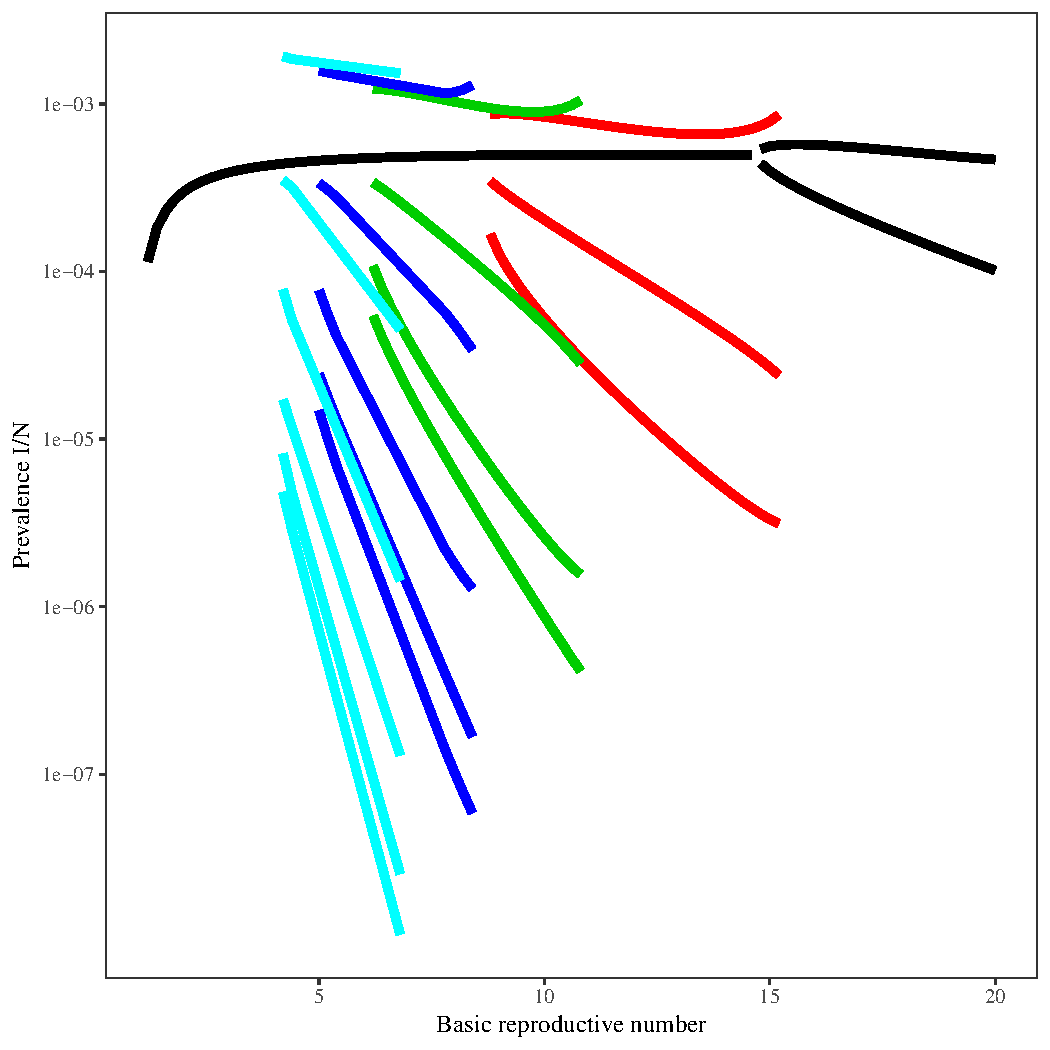
\includegraphics[width=\maxwidth]{figure/bifur_g-1} 

\end{knitrout}

\section{Probability of coherence in the deterministic model}
Before going into the bulk of the deterministic model section, we load a few useful functions which will be used throughout. The first is a function to calculate the incoherence measure defined in the main paper:
Let $\vec{I} (t) = (I_1(t), \dots, I_n(t))$ denote the number of individuals infected at time $t$ in patches $k = 1, \dots, n$. We then define incoherence $\delta$ at time $t$ as
$$
\delta(t) = || \vec{I}(t) - \langle \vec{I} (t) \rangle \vec{e}||_2,
$$
where $\langle \vec{I} (t) \rangle = \sum_{k=1}^n I_k(t) / n$ denotes the mean prevalence among the patches at time $t$, and $\vec{e} = (1, \dots, 1)$.

\begin{knitrout}
\definecolor{shadecolor}{rgb}{0.969, 0.969, 0.969}\color{fgcolor}\begin{kframe}
\begin{alltt}
\hlcom{# coherence metric calculation}
\hlstd{coherence_calc} \hlkwb{<-} \hlkwa{function}\hlstd{(}\hlkwc{x}\hlstd{) \{}
    \hlkwd{norm}\hlstd{(x} \hlopt{-} \hlkwd{rep}\hlstd{(}\hlkwd{mean}\hlstd{(x),} \hlkwd{length}\hlstd{(x)),} \hlkwc{type} \hlstd{=} \hlstr{"2"}\hlstd{)}
\hlstd{\}}
\end{alltt}
\end{kframe}
\end{knitrout}

Below is a function that generates random initial conditions with $0 < S_k < 0.1 N$, and $0 < I_k < 0.0001 N$ for each patch as described Earn et al. (2000): A Simple Model for Complex Dynamical Transitions in Epidemics.
\begin{knitrout}
\definecolor{shadecolor}{rgb}{0.969, 0.969, 0.969}\color{fgcolor}\begin{kframe}
\begin{alltt}
\hlstd{r.init.science} \hlkwb{<-} \hlkwa{function}\hlstd{(}\hlkwc{m}\hlstd{) \{}
    \hlstd{initial} \hlkwb{<-} \hlkwd{list}\hlstd{(}\hlkwc{S} \hlstd{=} \hlkwd{runif}\hlstd{(m,} \hlnum{0}\hlstd{,} \hlnum{0.1} \hlopt{*} \hlstd{base.params}\hlopt{$}\hlstd{pop))}
    \hlstd{initial}\hlopt{$}\hlstd{I} \hlkwb{<-} \hlkwd{runif}\hlstd{(m,} \hlnum{0}\hlstd{,} \hlnum{1e-04} \hlopt{*} \hlstd{base.params}\hlopt{$}\hlstd{pop)}
    \hlstd{initial}\hlopt{$}\hlstd{R} \hlkwb{<-} \hlkwd{rep}\hlstd{(base.params}\hlopt{$}\hlstd{pop, m)} \hlopt{-} \hlstd{initial}\hlopt{$}\hlstd{S} \hlopt{-} \hlstd{initial}\hlopt{$}\hlstd{I}
    \hlstd{initial}
\hlstd{\}}
\end{alltt}
\end{kframe}
\end{knitrout}

Lastly, we have a function that returns the results of the model simulation (from the \texttt{.cpp} file) in a convenient format.
\begin{knitrout}
\definecolor{shadecolor}{rgb}{0.969, 0.969, 0.969}\color{fgcolor}\begin{kframe}
\begin{alltt}
\hlstd{run_SIR} \hlkwb{<-} \hlkwa{function}\hlstd{(}\hlkwc{p}\hlstd{,} \hlkwc{init}\hlstd{,} \hlkwc{m}\hlstd{,} \hlkwc{seas}\hlstd{) \{}
    \hlcom{# get number of patches}
    \hlstd{n} \hlkwb{<-} \hlkwd{nrow}\hlstd{(m)}

    \hlcom{# Run the model}
    \hlstd{raw.result} \hlkwb{<-} \hlkwd{SIRmodel_npatch}\hlstd{(p, init, m, seas)}

    \hlcom{# Initialize result data frame}
    \hlstd{result} \hlkwb{<-} \hlkwd{data_frame}\hlstd{(}\hlkwc{t} \hlstd{= raw.result}\hlopt{$}\hlstd{time)}

    \hlcom{# Pull results}
    \hlstd{S} \hlkwb{<-} \hlstd{raw.result}\hlopt{$}\hlstd{S}
    \hlstd{I} \hlkwb{<-} \hlstd{raw.result}\hlopt{$}\hlstd{I}
    \hlstd{R} \hlkwb{<-} \hlstd{raw.result}\hlopt{$}\hlstd{R}

    \hlcom{# Change column names}
    \hlkwd{colnames}\hlstd{(S)} \hlkwb{<-} \hlkwd{str_c}\hlstd{(}\hlstr{"S"}\hlstd{,} \hlnum{1}\hlopt{:}\hlstd{n)}
    \hlkwd{colnames}\hlstd{(I)} \hlkwb{<-} \hlkwd{str_c}\hlstd{(}\hlstr{"I"}\hlstd{,} \hlnum{1}\hlopt{:}\hlstd{n)}
    \hlkwd{colnames}\hlstd{(R)} \hlkwb{<-} \hlkwd{str_c}\hlstd{(}\hlstr{"R"}\hlstd{,} \hlnum{1}\hlopt{:}\hlstd{n)}

    \hlcom{# Combine data frames}
    \hlkwd{cbind}\hlstd{(result, S, I, R)}
\hlstd{\}}
\end{alltt}
\end{kframe}
\end{knitrout}
Here we check if the data file corresponding to $m = 0.0001$ is present. If it is, then we load that file, and if it isn't, then we run the simulation that creates that file. Note that loading in the file will save a lot of time and if it is missing, we strongly recommend you get the file from us. Here we only show the code that loads data corresponding to $m =0.0001$, but the code for the remaining $m$ values (0.001, 0.01, 0.1, 0.5) are similar and therefore hidden.

You may be asking why we run all of these separately. This was to split up the computational load among our measly laptops. The $m$ values were split up as follows (by assigning the \texttt{mvec} vector accordingly: 
\begin{itemize}
\item \texttt{mvec = 0.0001} (assigned to \texttt{df1})
\item \texttt{mvec = c(0.001, 0.01)} (assigned to \texttt{df2})
\item \texttt{mvec = c(0.1, 0.5)} (assigned to \texttt{df3})
\end{itemize} 

For each $m$ value we test 100 random initial conditions and run the model for 100 years. Then we record the average incoherence value in the last 2 years and the last 5 years of the simulation for each initial condition.

\begin{knitrout}
\definecolor{shadecolor}{rgb}{0.969, 0.969, 0.969}\color{fgcolor}\begin{kframe}
\begin{alltt}
\hlkwa{if} \hlstd{(}\hlkwd{file.exists}\hlstd{(}\hlstr{"coherence_m0.0001.rda"}\hlstd{)) \{}
    \hlkwd{load}\hlstd{(}\hlstr{"coherence_m0.0001.rda"}\hlstd{)}
    \hlstd{df1} \hlkwb{<-} \hlstd{reslist}
\hlstd{\}} \hlkwa{else} \hlstd{\{}
    \hlstd{nsim} \hlkwb{<-} \hlnum{100}
    \hlstd{R0vec} \hlkwb{<-} \hlkwd{seq}\hlstd{(}\hlnum{1}\hlstd{,} \hlnum{20}\hlstd{,} \hlkwc{by} \hlstd{=} \hlnum{0.4}\hlstd{)}
    \hlstd{mvec} \hlkwb{<-} \hlkwd{c}\hlstd{(}\hlnum{1e-04}\hlstd{)}
    \hlstd{reslist} \hlkwb{<-} \hlkwd{vector}\hlstd{(}\hlstr{"list"}\hlstd{,} \hlkwd{length}\hlstd{(mvec))}
    \hlkwd{set.seed}\hlstd{(}\hlnum{101}\hlstd{)}
    \hlkwa{for} \hlstd{(m} \hlkwa{in} \hlstd{mvec) \{}
        \hlstd{M} \hlkwb{<-} \hlkwd{matrix}\hlstd{(}\hlkwd{c}\hlstd{(}\hlnum{1} \hlopt{-} \hlstd{m, m, m,} \hlnum{1} \hlopt{-} \hlstd{m),} \hlnum{2}\hlstd{,} \hlnum{2}\hlstd{)}
        \hlstd{subreslist} \hlkwb{<-} \hlkwd{vector}\hlstd{(}\hlstr{"list"}\hlstd{,} \hlkwd{length}\hlstd{(R0vec))}
        \hlkwa{for} \hlstd{(R} \hlkwa{in} \hlstd{R0vec) \{}
            \hlkwd{print}\hlstd{(}\hlkwd{paste}\hlstd{(m, R,} \hlkwc{sep} \hlstd{=} \hlstr{","}\hlstd{))}

            \hlstd{pp} \hlkwb{<-} \hlstd{base.params}
            \hlstd{pp[[}\hlstr{"R0"}\hlstd{]]} \hlkwb{<-} \hlstd{R}

            \hlstd{subsubreslist} \hlkwb{<-} \hlkwd{vector}\hlstd{(}\hlstr{"list"}\hlstd{, nsim)}

            \hlkwa{for} \hlstd{(i} \hlkwa{in} \hlnum{1}\hlopt{:}\hlstd{nsim) \{}

                \hlstd{init} \hlkwb{<-} \hlkwd{r.init.science}\hlstd{(}\hlnum{2}\hlstd{)}
                \hlstd{df} \hlkwb{<-} \hlkwd{run_SIR}\hlstd{(pp, init, M, term_time)}

                \hlstd{incoherence2} \hlkwb{<-} \hlkwd{apply}\hlstd{(df[(}\hlkwd{nrow}\hlstd{(df)} \hlopt{-} \hlnum{2} \hlopt{*} \hlnum{365}\hlstd{)}\hlopt{:}\hlkwd{nrow}\hlstd{(df),} \hlkwd{c}\hlstd{(}\hlstr{"I1"}\hlstd{,}
                  \hlstr{"I2"}\hlstd{)],} \hlnum{1}\hlstd{, coherence_calc)} \hlopt \hlkwd{mean}\hlstd{()}
                \hlstd{incoherence5} \hlkwb{<-} \hlkwd{apply}\hlstd{(df[(}\hlkwd{nrow}\hlstd{(df)} \hlopt{-} \hlnum{5} \hlopt{*} \hlnum{365}\hlstd{)}\hlopt{:}\hlkwd{nrow}\hlstd{(df),} \hlkwd{c}\hlstd{(}\hlstr{"I1"}\hlstd{,}
                  \hlstr{"I2"}\hlstd{)],} \hlnum{1}\hlstd{, coherence_calc)} \hlopt \hlkwd{mean}\hlstd{()}

                \hlstd{subsubreslist[[i]]} \hlkwb{<-} \hlkwd{data_frame}\hlstd{(}\hlkwc{S01} \hlstd{= init}\hlopt{$}\hlstd{S[}\hlnum{1}\hlstd{],} \hlkwc{S02} \hlstd{= init}\hlopt{$}\hlstd{S[}\hlnum{2}\hlstd{],}
                  \hlkwc{I01} \hlstd{= init}\hlopt{$}\hlstd{I[}\hlnum{1}\hlstd{],} \hlkwc{I02} \hlstd{= init}\hlopt{$}\hlstd{I[}\hlnum{2}\hlstd{],} \hlkwc{R0} \hlstd{= R,} \hlkwc{incoherence2} \hlstd{= incoherence2,}
                  \hlkwc{incoherence5} \hlstd{= incoherence5)}
            \hlstd{\}}
            \hlstd{subreslist[[}\hlkwd{which}\hlstd{(R0vec} \hlopt{==} \hlstd{R)]]} \hlkwb{<-} \hlkwd{do.call}\hlstd{(}\hlstr{"rbind"}\hlstd{, subsubreslist)}
        \hlstd{\}}

        \hlstd{ss} \hlkwb{<-} \hlkwd{do.call}\hlstd{(}\hlstr{"rbind"}\hlstd{, subreslist)}
        \hlstd{ss}\hlopt{$}\hlstd{m} \hlkwb{<-} \hlstd{m}
        \hlstd{reslist[[}\hlkwd{which}\hlstd{(mvec} \hlopt{==} \hlstd{m)]]} \hlkwb{<-} \hlstd{ss}
    \hlstd{\}}
\hlstd{\}}
\end{alltt}
\end{kframe}
\end{knitrout}






Here we combine the three data frames that consist of the data for different $m$ values, and then we construct the plot showing the probability of coherence in the main paper. This particular figure uses a threshold of average incoherence < 100 in the last 2 years.

\begin{knitrout}
\definecolor{shadecolor}{rgb}{0.969, 0.969, 0.969}\color{fgcolor}\begin{kframe}
\begin{alltt}
\hlstd{R0df} \hlkwb{<-} \hlkwd{bind_rows}\hlstd{(df1, df2, df3)} \hlopt \hlkwd{group_by}\hlstd{(R0, m)} \hlopt \hlkwd{summarize}\hlstd{(}\hlkwc{prob.coherence} \hlstd{=} \hlkwd{length}\hlstd{(}\hlkwd{which}\hlstd{((incoherence2} \hlopt{<}
    \hlnum{100}\hlstd{)))}\hlopt{/}\hlnum{100}\hlstd{)} \hlopt \hlkwd{mutate}\hlstd{(}\hlkwc{m.factor} \hlstd{=} \hlkwd{as.factor}\hlstd{(m))}

\hlstd{bifur_df_norm} \hlkwb{<-} \hlstd{bifur_df} \hlopt \hlkwd{mutate}\hlstd{(}\hlkwc{lp} \hlstd{=} \hlkwd{log}\hlstd{(prevalence))} \hlopt \hlkwd{mutate}\hlstd{(}\hlkwc{nlp} \hlstd{= lp} \hlopt{-}
    \hlkwd{min}\hlstd{(lp))} \hlopt \hlkwd{mutate}\hlstd{(}\hlkwc{nlp} \hlstd{= nlp}\hlopt{/}\hlkwd{max}\hlstd{(nlp))}

\hlkwd{levels}\hlstd{(R0df}\hlopt{$}\hlstd{m.factor)} \hlkwb{<-} \hlkwd{c}\hlstd{(}\hlstr{"m = 0.0001"}\hlstd{,} \hlstr{"m = 0.001"}\hlstd{,} \hlstr{"m = 0.01"}\hlstd{,} \hlstr{"m = 0.1"}\hlstd{,}
    \hlstr{"m = 0.5"}\hlstd{)}

\hlstd{gprob.main} \hlkwb{<-} \hlkwd{ggplot}\hlstd{(R0df)} \hlopt{+} \hlkwd{geom_line}\hlstd{(}\hlkwd{aes}\hlstd{(R0, prob.coherence),} \hlkwc{size} \hlstd{=} \hlnum{1}\hlstd{)} \hlopt{+}
    \hlkwd{facet_wrap}\hlstd{(}\hlopt{~}\hlstd{m.factor,} \hlkwc{ncol} \hlstd{=} \hlnum{2}\hlstd{)} \hlopt{+} \hlkwd{geom_path}\hlstd{(}\hlkwc{data} \hlstd{= bifur_df_norm,} \hlkwd{aes}\hlstd{(R0,}
    \hlstd{nlp,} \hlkwc{group} \hlstd{=} \hlkwd{interaction}\hlstd{(i, j, sim),} \hlkwc{col} \hlstd{=} \hlkwd{factor}\hlstd{(i)),} \hlkwc{alpha} \hlstd{=} \hlnum{0.5}\hlstd{)} \hlopt{+} \hlkwd{labs}\hlstd{(}\hlkwc{x} \hlstd{=} \hlstr{"Reproductive number"}\hlstd{,}
    \hlkwc{y} \hlstd{=} \hlstr{"Probability of coherence"}\hlstd{)} \hlopt{+} \hlkwd{scale_color_manual}\hlstd{(}\hlkwc{values} \hlstd{=} \hlkwd{c}\hlstd{(}\hlnum{1}\hlstd{,} \hlnum{1}\hlstd{,} \hlnum{2}\hlstd{,}
    \hlnum{3}\hlstd{,} \hlnum{4}\hlstd{,} \hlnum{5}\hlstd{,} \hlnum{6}\hlstd{))} \hlopt{+} \hlkwd{theme}\hlstd{(}\hlkwc{legend.position} \hlstd{=} \hlstr{"none"}\hlstd{)}

\hlstd{gprob.main}
\end{alltt}
\end{kframe}
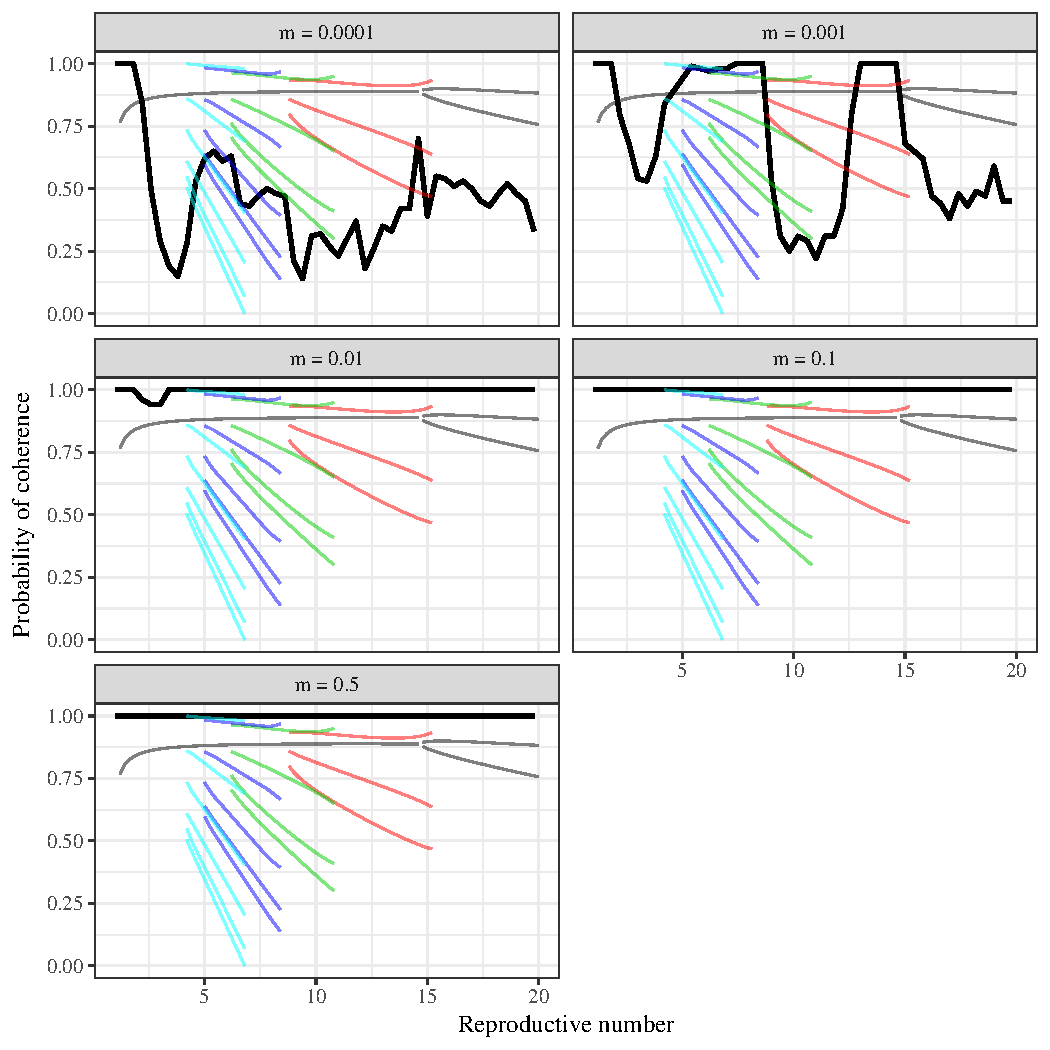
\includegraphics[width=\maxwidth]{figure/coherenceplot-main-1} 

\end{knitrout}

Next, we calculate the mean probabilities of coherence for mixing values of $0.01\%$ ($m=0.0001$), $0.1\%$ ($m=0.001$), and $1\%$ ($m=0.01$) across all basic reproductive number values. 

\begin{knitrout}
\definecolor{shadecolor}{rgb}{0.969, 0.969, 0.969}\color{fgcolor}\begin{kframe}
\begin{alltt}
\hlcom{# for 0.0001}
\hlstd{R0df_0.0001} \hlkwb{<-} \hlkwd{bind_rows}\hlstd{(df1[[}\hlnum{1}\hlstd{]])} \hlopt \hlkwd{group_by}\hlstd{(R0, m)} \hlopt \hlkwd{summarize}\hlstd{(}\hlkwc{prob.coherence} \hlstd{=} \hlkwd{length}\hlstd{(}\hlkwd{which}\hlstd{((incoherence2} \hlopt{<}
    \hlnum{100}\hlstd{)))}\hlopt{/}\hlnum{100}\hlstd{)}
\hlkwd{str_c}\hlstd{(}\hlstr{"The mean for m=0.0001 is "}\hlstd{,} \hlkwd{mean}\hlstd{(R0df_0.0001}\hlopt{$}\hlstd{prob.coherence))}
\end{alltt}
\begin{verbatim}
## [1] "The mean for m=0.0001 is 0.459166666666667"
\end{verbatim}
\begin{alltt}
\hlcom{# for 0.001}
\hlstd{R0df_0.001} \hlkwb{<-} \hlstd{R0df} \hlkwb{<-} \hlkwd{bind_rows}\hlstd{(df2[[}\hlnum{1}\hlstd{]])} \hlopt \hlkwd{group_by}\hlstd{(R0, m)} \hlopt \hlkwd{summarize}\hlstd{(}\hlkwc{prob.coherence} \hlstd{=} \hlkwd{length}\hlstd{(}\hlkwd{which}\hlstd{((incoherence2} \hlopt{<}
    \hlnum{100}\hlstd{)))}\hlopt{/}\hlnum{100}\hlstd{)}
\hlkwd{str_c}\hlstd{(}\hlstr{"The mean for m=0.001 is "}\hlstd{,} \hlkwd{mean}\hlstd{(R0df_0.001}\hlopt{$}\hlstd{prob.coherence))}
\end{alltt}
\begin{verbatim}
## [1] "The mean for m=0.001 is 0.689375"
\end{verbatim}
\begin{alltt}
\hlcom{# for 0.01}
\hlstd{R0df_0.01} \hlkwb{<-} \hlstd{R0df} \hlkwb{<-} \hlkwd{bind_rows}\hlstd{(df2[[}\hlnum{2}\hlstd{]])} \hlopt \hlkwd{group_by}\hlstd{(R0, m)} \hlopt \hlkwd{summarize}\hlstd{(}\hlkwc{prob.coherence} \hlstd{=} \hlkwd{length}\hlstd{(}\hlkwd{which}\hlstd{((incoherence2} \hlopt{<}
    \hlnum{100}\hlstd{)))}\hlopt{/}\hlnum{100}\hlstd{)}
\hlkwd{str_c}\hlstd{(}\hlstr{"The mean for m=0.01 is "}\hlstd{,} \hlkwd{mean}\hlstd{(R0df_0.01}\hlopt{$}\hlstd{prob.coherence))}
\end{alltt}
\begin{verbatim}
## [1] "The mean for m=0.01 is 0.996666666666667"
\end{verbatim}
\end{kframe}
\end{knitrout}
\subsection{Choice of incoherence threshold}
Here we demonstrate that we obtain similar coherence probabilities even with different choices of threshold. This demonstrates that our observed results and inferences aren't sensitive to our choice of coherence threshold.

Threshold of 10:

\begin{knitrout}
\definecolor{shadecolor}{rgb}{0.969, 0.969, 0.969}\color{fgcolor}
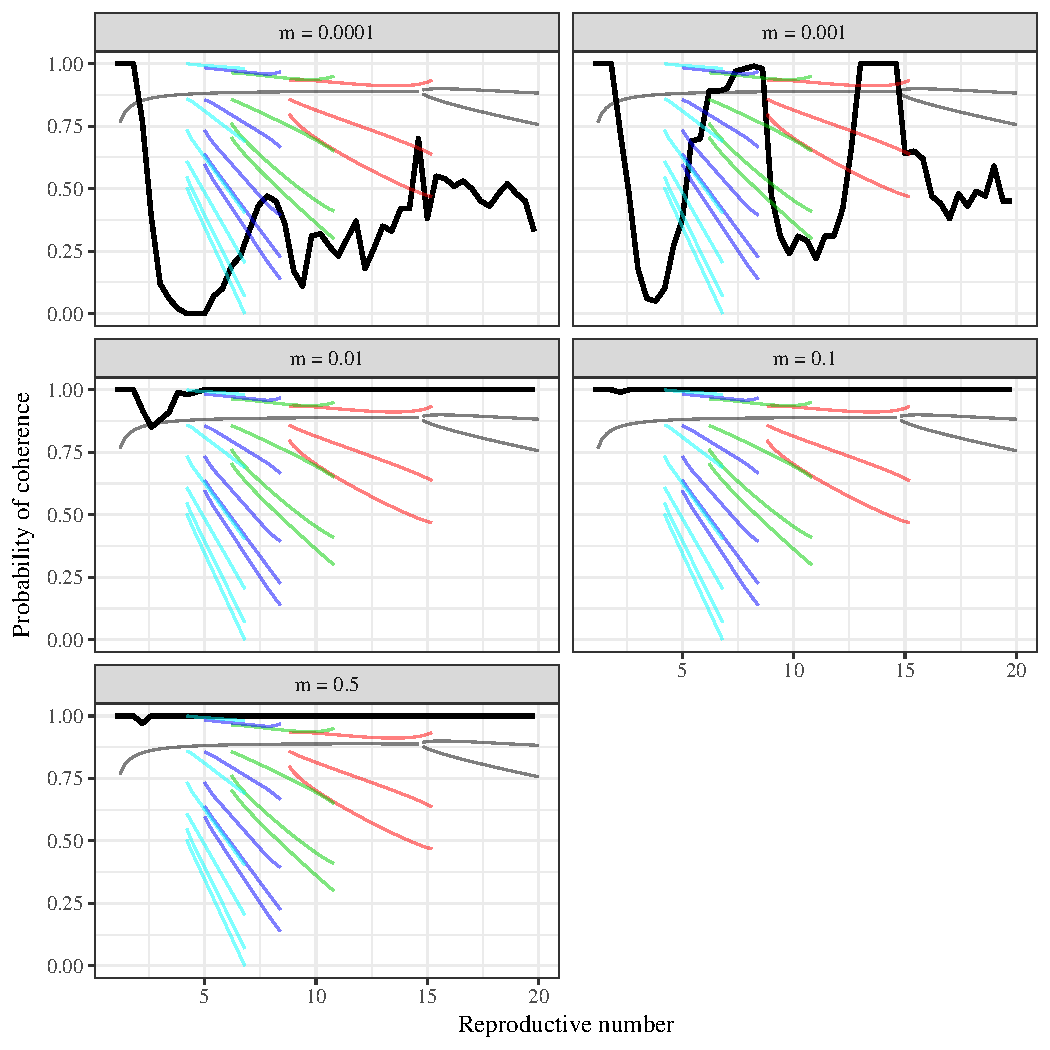
\includegraphics[width=\maxwidth]{figure/coherenceplot-5-1} 

\end{knitrout}

Threshold of 200:

\begin{knitrout}
\definecolor{shadecolor}{rgb}{0.969, 0.969, 0.969}\color{fgcolor}
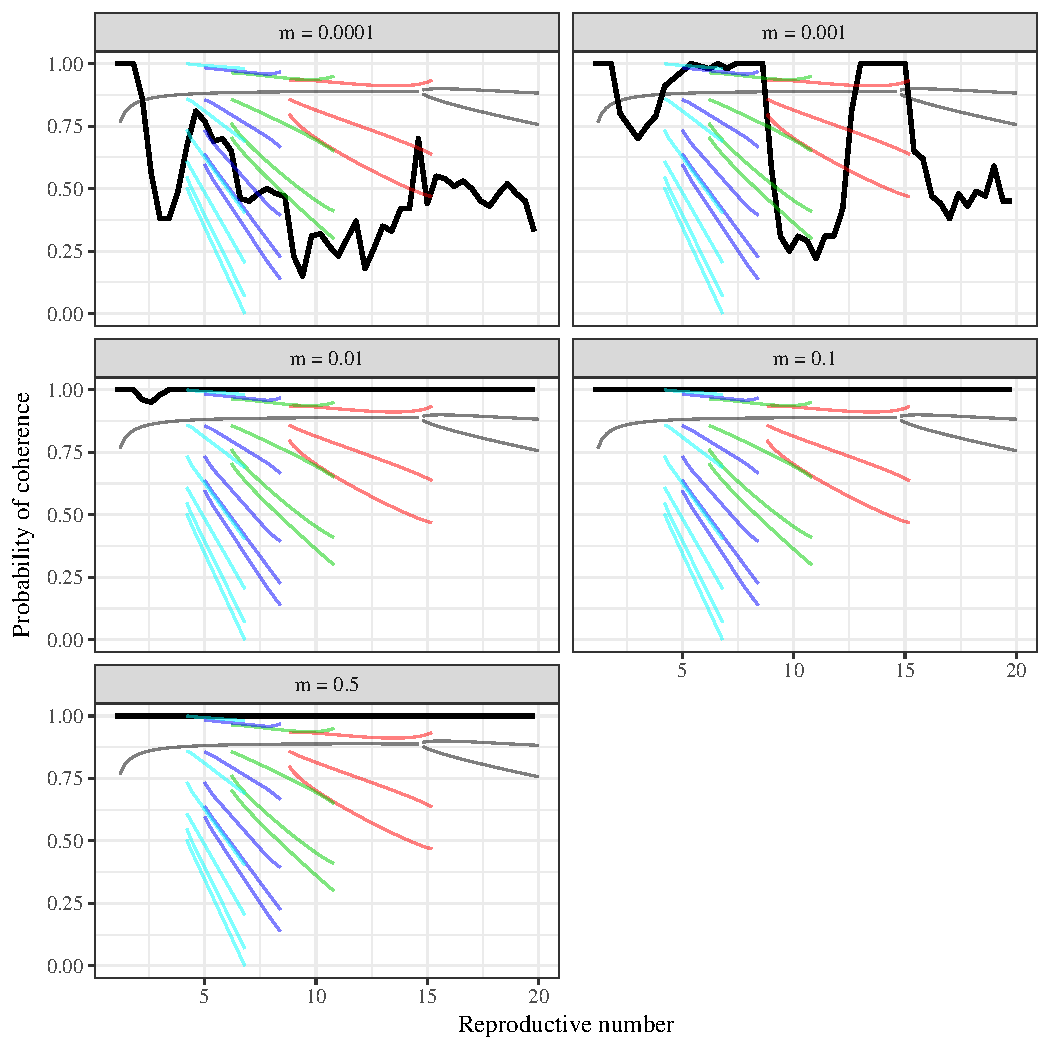
\includegraphics[width=\maxwidth]{figure/coherenceplot-200-1} 

\end{knitrout}

\subsection{Coherence in the last 5 years}
Here we show that our inferences are also not sensitive to whether we measure the average incoherence over the last 2 or 5 years. The plot in the main paper uses a last-2-year measure of average incoherence, but we see below that changing this to the last 5 years (with the same incoherence < 100 threshold) results in similar behaviour.

\begin{knitrout}
\definecolor{shadecolor}{rgb}{0.969, 0.969, 0.969}\color{fgcolor}
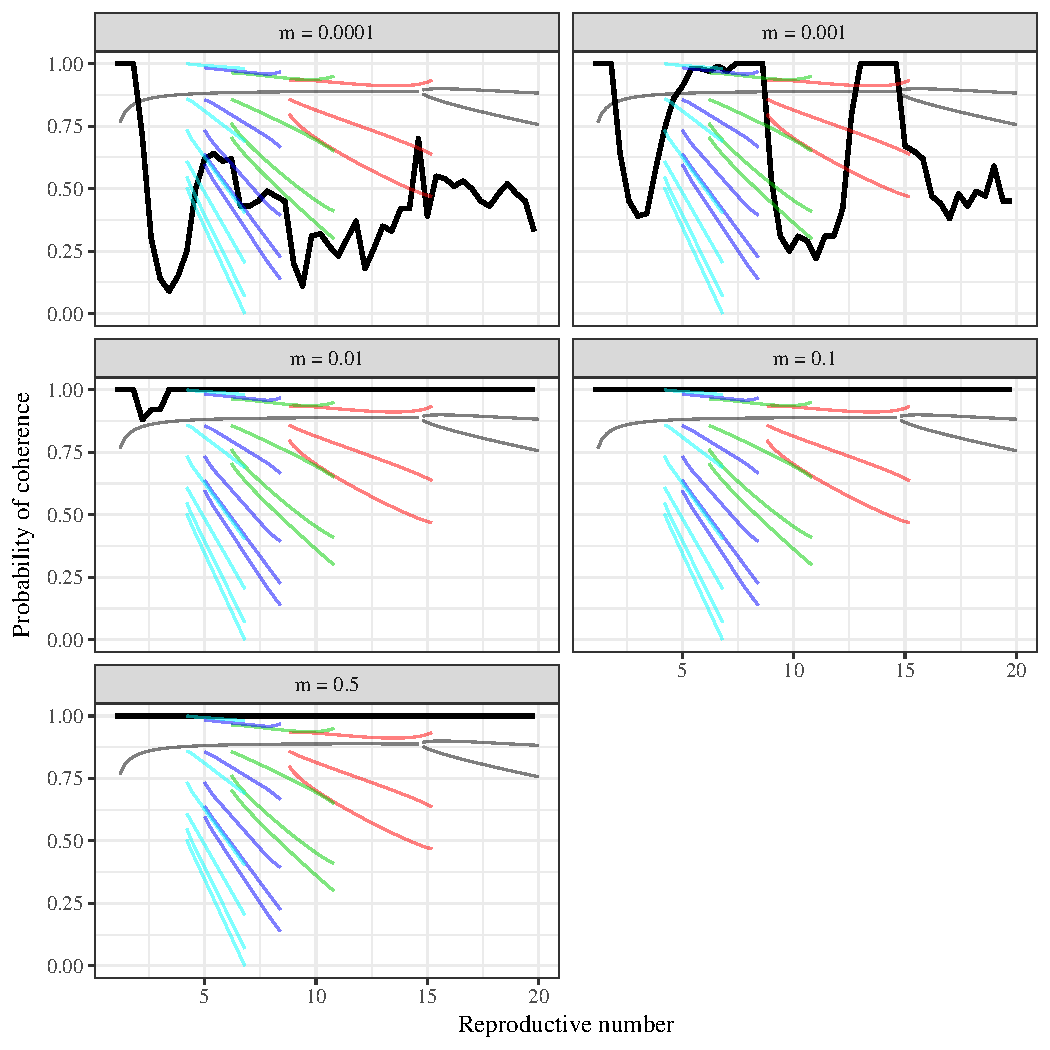
\includegraphics[width=\maxwidth]{figure/coherenceplot-5year-1} 

\end{knitrout}

\section{Synchrony and asynchrony in stochastic model}

We observe stretches of both synchrony and asynchrony in simulated trajectory for the stochastic model. We let $\R_0 = 17$ and let the mixing proportion be given by 0.1\% ($m = 0.001$). Our initial conditions are given by the endemic equilibrium, and the rest of our parameters are taken from the base parameters list. We observe the change from synchronous behaviour to asynchronous behaviour in Figure 2, which can be reproduced using the following code:

\begin{knitrout}
\definecolor{shadecolor}{rgb}{0.969, 0.969, 0.969}\color{fgcolor}\begin{kframe}
\begin{alltt}
\hlstd{pp3} \hlkwb{<-} \hlstd{base.params}
\hlstd{pp3[[}\hlstr{"R0"}\hlstd{]]} \hlkwb{<-} \hlnum{17.0}

\hlstd{init} \hlkwb{<-} \hlkwd{initfun}\hlstd{(pp3,} \hlnum{2}\hlstd{, T)}
\hlstd{m} \hlkwb{<-} \hlnum{0.001}
\hlstd{M} \hlkwb{<-} \hlkwd{matrix}\hlstd{(}\hlkwd{c}\hlstd{(}\hlnum{1}\hlopt{-}\hlstd{m, m, m,} \hlnum{1}\hlopt{-}\hlstd{m),} \hlnum{2}\hlstd{,} \hlnum{2}\hlstd{)}

\hlkwd{set.seed}\hlstd{(}\hlnum{10}\hlstd{)}
\hlstd{df4} \hlkwb{<-} \hlkwd{SIRmodel_npatch_stochastic}\hlstd{(pp3, init, M, term_time)}
\end{alltt}


{\ttfamily\noindent\bfseries\color{errorcolor}{\#\# Error in SIRmodel\_npatch\_stochastic(pp3, init, M, term\_time): could not find function "{}SIRmodel\_npatch\_stochastic"{}}}\begin{alltt}
\hlstd{simdf3} \hlkwb{<-} \hlkwd{list}\hlstd{(}
    \hlkwc{patch1}\hlstd{=}\hlkwd{data.frame}\hlstd{(}
        \hlkwc{time}\hlstd{=df4}\hlopt{$}\hlstd{time,}
        \hlkwc{I}\hlstd{=df4}\hlopt{$}\hlstd{I[,}\hlnum{1}\hlstd{]}
    \hlstd{),}
    \hlkwc{patch2}\hlstd{=}\hlkwd{data.frame}\hlstd{(}
        \hlkwc{time}\hlstd{=df4}\hlopt{$}\hlstd{time,}
        \hlkwc{I}\hlstd{=df4}\hlopt{$}\hlstd{I[,}\hlnum{2}\hlstd{]}
    \hlstd{)}
\hlstd{)} \hlopt
    \hlkwd{bind_rows}\hlstd{(}\hlkwc{.id}\hlstd{=}\hlstr{"patch"}\hlstd{)} \hlopt
    \hlkwd{gather}\hlstd{(key, value,} \hlopt{-}\hlstd{time,} \hlopt{-}\hlstd{patch)} \hlopt
    \hlkwd{filter}\hlstd{(time} \hlopt{>} \hlnum{60}\hlstd{, time} \hlopt{<} \hlnum{85}\hlstd{)}
\end{alltt}


{\ttfamily\noindent\bfseries\color{errorcolor}{\#\# Error in data.frame(time = df4\$time, I = df4\$I[, 1]): object 'df4' not found}}\begin{alltt}
\hlstd{gex} \hlkwb{<-} \hlkwd{ggplot}\hlstd{(simdf3)} \hlopt{+}
    \hlkwd{geom_line}\hlstd{(}\hlkwd{aes}\hlstd{(time, value,} \hlkwc{col}\hlstd{=patch),} \hlkwc{lwd}\hlstd{=}\hlnum{1.1}\hlstd{)} \hlopt{+}
    \hlkwd{scale_x_continuous}\hlstd{(}\hlstr{"Time (years)"}\hlstd{,} \hlkwc{expand}\hlstd{=}\hlkwd{c}\hlstd{(}\hlnum{0}\hlstd{,} \hlnum{0}\hlstd{))} \hlopt{+}
    \hlkwd{scale_y_continuous}\hlstd{(}\hlstr{"Prevalence"}\hlstd{)} \hlopt{+}
    \hlkwd{scale_color_manual}\hlstd{(}\hlkwc{labels}\hlstd{=}\hlkwd{c}\hlstd{(}\hlstr{"Patch 1"}\hlstd{,} \hlstr{"Patch 2"}\hlstd{),} \hlkwc{values}\hlstd{=}\hlkwd{c}\hlstd{(}\hlstr{"#D55E00"}\hlstd{,} \hlstr{"#0072B2"}\hlstd{))} \hlopt{+}
    \hlkwd{theme}\hlstd{(}
        \hlkwc{panel.grid} \hlstd{=} \hlkwd{element_blank}\hlstd{(),}
        \hlkwc{legend.title} \hlstd{=} \hlkwd{element_blank}\hlstd{(),}
        \hlkwc{legend.position} \hlstd{=} \hlkwd{c}\hlstd{(}\hlnum{0.1}\hlstd{,} \hlnum{0.84}\hlstd{),}
        \hlkwc{strip.text} \hlstd{=} \hlkwd{element_text}\hlstd{(}\hlkwc{size}\hlstd{=}\hlnum{25}\hlstd{))}
\end{alltt}


{\ttfamily\noindent\bfseries\color{errorcolor}{\#\# Error in ggplot(simdf3): object 'simdf3' not found}}\begin{alltt}
\hlkwd{plot}\hlstd{(gex)}
\end{alltt}


{\ttfamily\noindent\bfseries\color{errorcolor}{\#\# Error in plot(gex): object 'gex' not found}}\end{kframe}
\end{knitrout}


\section{Probability of extinction}

\subsection{Factorial simulation}

Here, we vary $\R_0$ from 1 to 20 by 0.2 steps and simulate the stochastic model 100 times for each combination of $\R_0$ and mixing proportion $m$.
Here, we do not use random initial conditions as it may lead to exaggeration of global extinction probability (some initial conditions may lead to immediate extinction without a start of an epidemic).
Instead, we start from the endemic equilibrium.
Once again, as this simulation takes approximately 11 hours, we load a saved file instead.

\begin{knitrout}
\definecolor{shadecolor}{rgb}{0.969, 0.969, 0.969}\color{fgcolor}\begin{kframe}
\begin{alltt}
\hlkwa{if} \hlstd{(}\hlkwd{file.exists}\hlstd{(}\hlstr{"stochastic.rda"}\hlstd{)) \{}
    \hlkwd{load}\hlstd{(}\hlstr{"stochastic.rda"}\hlstd{)}
\hlstd{\}} \hlkwa{else} \hlstd{\{}
    \hlstd{nsim} \hlkwb{<-} \hlnum{100}
    \hlstd{R0vec} \hlkwb{<-} \hlkwd{seq}\hlstd{(}\hlnum{1}\hlstd{,} \hlnum{20}\hlstd{,} \hlkwc{by}\hlstd{=}\hlnum{0.2}\hlstd{)}
    \hlstd{mvec} \hlkwb{<-} \hlkwd{c}\hlstd{(}\hlnum{0.001}\hlstd{,} \hlnum{0.01}\hlstd{,} \hlnum{0.1}\hlstd{,} \hlnum{0.5}\hlstd{)}

    \hlstd{reslist} \hlkwb{<-} \hlkwd{vector}\hlstd{(}\hlstr{'list'}\hlstd{,} \hlkwd{length}\hlstd{(mvec))}
    \hlkwd{set.seed}\hlstd{(}\hlnum{101}\hlstd{)}
    \hlkwa{for} \hlstd{(m} \hlkwa{in} \hlstd{mvec) \{}

        \hlstd{M} \hlkwb{<-} \hlkwd{matrix}\hlstd{(}\hlkwd{c}\hlstd{(}\hlnum{1}\hlopt{-}\hlstd{m, m, m,} \hlnum{1}\hlopt{-}\hlstd{m),} \hlnum{2}\hlstd{,} \hlnum{2}\hlstd{)}
        \hlstd{subreslist} \hlkwb{<-} \hlkwd{vector}\hlstd{(}\hlstr{'list'}\hlstd{,} \hlkwd{length}\hlstd{(R0vec))}

        \hlkwa{for} \hlstd{(R} \hlkwa{in} \hlstd{R0vec) \{}
            \hlstd{pp} \hlkwb{<-} \hlstd{base.params}
            \hlstd{pp[[}\hlstr{"R0"}\hlstd{]]} \hlkwb{<-} \hlstd{R}

            \hlstd{subsubreslist} \hlkwb{<-} \hlkwd{vector}\hlstd{(}\hlstr{'list'}\hlstd{, nsim)}
            \hlkwa{for} \hlstd{(i} \hlkwa{in} \hlnum{1}\hlopt{:}\hlstd{nsim) \{}
                \hlstd{init} \hlkwb{<-} \hlkwd{initfun}\hlstd{(pp,} \hlnum{2}\hlstd{, T)}
                \hlstd{df} \hlkwb{<-} \hlkwd{SIRmodel_npatch_stochastic}\hlstd{(base.params, init, M, term_time)}
                \hlstd{zero1} \hlkwb{<-} \hlkwd{which}\hlstd{(df}\hlopt{$}\hlstd{I[,}\hlnum{1}\hlstd{]}\hlopt{==}\hlnum{0}\hlstd{)}
                \hlstd{zero2} \hlkwb{<-} \hlkwd{which}\hlstd{(df}\hlopt{$}\hlstd{I[,}\hlnum{2}\hlstd{]}\hlopt{==}\hlnum{0}\hlstd{)}
                \hlstd{subsubreslist[[i]]} \hlkwb{<-} \hlkwd{data.frame}\hlstd{(}
                    \hlkwc{sim}\hlstd{=i,}
                    \hlkwc{R0}\hlstd{=R,}
                    \hlkwc{local}\hlstd{=(}\hlkwd{any}\hlstd{(df}\hlopt{$}\hlstd{I[,}\hlnum{1}\hlstd{]}\hlopt{==}\hlnum{0}\hlstd{)} \hlopt{||} \hlkwd{any}\hlstd{(df}\hlopt{$}\hlstd{I[,}\hlnum{2}\hlstd{]}\hlopt{==}\hlnum{0}\hlstd{)),}
                    \hlkwc{global}\hlstd{=(}\hlkwd{any}\hlstd{(df}\hlopt{$}\hlstd{I[,}\hlnum{1}\hlstd{]}\hlopt{==}\hlnum{0} \hlopt{&} \hlstd{df}\hlopt{$}\hlstd{I[,}\hlnum{2}\hlstd{]}\hlopt{==}\hlnum{0}\hlstd{)),}
                    \hlkwc{rescue1}\hlstd{=}\hlkwd{length}\hlstd{(}\hlkwd{which}\hlstd{(}\hlkwd{diff}\hlstd{(zero1)} \hlopt{!=} \hlnum{1}\hlstd{)),}
                    \hlkwc{rescue2}\hlstd{=}\hlkwd{length}\hlstd{(}\hlkwd{which}\hlstd{(}\hlkwd{diff}\hlstd{(zero2)} \hlopt{!=} \hlnum{1}\hlstd{))}
                \hlstd{)}
            \hlstd{\}}
            \hlstd{subreslist[[}\hlkwd{which}\hlstd{(R0vec}\hlopt{==}\hlstd{R)]]} \hlkwb{<-} \hlkwd{do.call}\hlstd{(}\hlstr{"rbind"}\hlstd{, subsubreslist)}
        \hlstd{\}}
        \hlstd{ss} \hlkwb{<-} \hlkwd{do.call}\hlstd{(}\hlstr{"rbind"}\hlstd{, subreslist)}
        \hlstd{ss}\hlopt{$}\hlstd{m} \hlkwb{<-} \hlstd{m}
        \hlstd{reslist[[}\hlkwd{which}\hlstd{(mvec}\hlopt{==}\hlstd{m)]]} \hlkwb{<-} \hlstd{ss}
    \hlstd{\}}
    \hlkwd{save}\hlstd{(}\hlstr{"reslist"}\hlstd{,} \hlkwc{file}\hlstd{=}\hlstr{"stochastic.rda"}\hlstd{)}
\hlstd{\}}
\end{alltt}
\end{kframe}
\end{knitrout}

\subsection{Plot}

Using the simulated file, we can plot the results of the simulation.
First, we clean up the data using \texttt{dplyr} and \texttt{tidyr} pacakge so that it can be used with a \texttt{ggplot} function.

\begin{knitrout}
\definecolor{shadecolor}{rgb}{0.969, 0.969, 0.969}\color{fgcolor}\begin{kframe}
\begin{alltt}
\hlstd{sdf} \hlkwb{<-} \hlstd{reslist} \hlopt
    \hlstd{bind_rows} \hlopt
    \hlkwd{group_by}\hlstd{(R0, m)} \hlopt
    \hlkwd{summarize}\hlstd{(}
        \hlkwc{local}\hlstd{=}\hlkwd{mean}\hlstd{(local),}
        \hlkwc{global}\hlstd{=}\hlkwd{mean}\hlstd{(global)}
    \hlstd{)} \hlopt
    \hlkwd{gather}\hlstd{(key, value,} \hlopt{-}\hlstd{R0,} \hlopt{-}\hlstd{m)} \hlopt
    \hlkwd{mutate}\hlstd{(}\hlkwc{m}\hlstd{=}\hlkwd{paste0}\hlstd{(}\hlstr{"m = "}\hlstd{, m),}
           \hlkwc{key}\hlstd{=}\hlkwd{factor}\hlstd{(key,} \hlkwc{levels}\hlstd{=}\hlkwd{c}\hlstd{(}\hlstr{"global"}\hlstd{,} \hlstr{"local"}\hlstd{),}
                      \hlkwc{labels}\hlstd{=}\hlkwd{c}\hlstd{(}\hlstr{"Global extinction"}\hlstd{,} \hlstr{"Local extinction"}\hlstd{)))}
\end{alltt}
\end{kframe}
\end{knitrout}

We are interested in comparing global and local extinction probabilities for measles parameters.
The following code demonstrates how to achieve appropriate statistics.

\begin{knitrout}
\definecolor{shadecolor}{rgb}{0.969, 0.969, 0.969}\color{fgcolor}\begin{kframe}
\begin{alltt}
\hlstd{sdf} \hlopt
    \hlkwd{filter}\hlstd{(R0} \hlopt{>} \hlnum{12.5}\hlstd{, R0} \hlopt{<=}\hlnum{18}\hlstd{, m}\hlopt{==}\hlstr{"m = 0.001"}\hlstd{)} \hlopt
    \hlkwd{group_by}\hlstd{(key)} \hlopt
    \hlkwd{summarize}\hlstd{(}
        \hlkwc{lwr}\hlstd{=}\hlkwd{range}\hlstd{(value)[}\hlnum{1}\hlstd{],}
        \hlkwc{upr}\hlstd{=}\hlkwd{range}\hlstd{(value)[}\hlnum{2}\hlstd{]}
    \hlstd{)}
\end{alltt}
\begin{verbatim}
## # A tibble: 2 x 3
##   key                 lwr   upr
##   <fct>             <dbl> <dbl>
## 1 Global extinction 0.    0.130
## 2 Local extinction  0.230 0.650
\end{verbatim}
\end{kframe}
\end{knitrout}

We are interested in comparing global extinction probabilities across different mixing proportions.
The following code demonstrates how to achieve appropriate statistics.

\begin{knitrout}
\definecolor{shadecolor}{rgb}{0.969, 0.969, 0.969}\color{fgcolor}\begin{kframe}
\begin{alltt}
\hlstd{sdf} \hlopt
    \hlkwd{filter}\hlstd{(R0} \hlopt{>} \hlnum{10}\hlstd{, key}\hlopt{==}\hlstr{"Global extinction"}\hlstd{)} \hlopt
    \hlkwd{group_by}\hlstd{(m)} \hlopt
    \hlkwd{summarize}\hlstd{(}
        \hlkwc{lwr}\hlstd{=}\hlkwd{range}\hlstd{(value)[}\hlnum{1}\hlstd{],}
        \hlkwc{upr}\hlstd{=}\hlkwd{range}\hlstd{(value)[}\hlnum{2}\hlstd{]}
    \hlstd{)}
\end{alltt}
\begin{verbatim}
## # A tibble: 4 x 3
##   m           lwr   upr
##   <chr>     <dbl> <dbl>
## 1 m = 0.001    0. 0.330
## 2 m = 0.01     0. 0.470
## 3 m = 0.1      0. 0.520
## 4 m = 0.5      0. 0.480
\end{verbatim}
\end{kframe}
\end{knitrout}

Before we plot the result of our stochastic simulation, we have to normalize the bifurcation diagram so that it can be layed below the probability diagram.

\begin{knitrout}
\definecolor{shadecolor}{rgb}{0.969, 0.969, 0.969}\color{fgcolor}\begin{kframe}
\begin{alltt}
\hlstd{bifur_df_norm} \hlkwb{<-} \hlstd{bifur_df} \hlopt
    \hlkwd{mutate}\hlstd{(}\hlkwc{lp}\hlstd{=}\hlkwd{log}\hlstd{(prevalence))} \hlopt
    \hlkwd{mutate}\hlstd{(}\hlkwc{nlp}\hlstd{=lp}\hlopt{-}\hlkwd{min}\hlstd{(lp))} \hlopt
    \hlkwd{mutate}\hlstd{(}\hlkwc{nlp}\hlstd{=nlp}\hlopt{/}\hlkwd{max}\hlstd{(nlp))}
\end{alltt}
\end{kframe}
\end{knitrout}

Finally, we generate the diagram of interest:

\begin{knitrout}
\definecolor{shadecolor}{rgb}{0.969, 0.969, 0.969}\color{fgcolor}\begin{kframe}
\begin{alltt}
\hlstd{gstoch} \hlkwb{<-} \hlkwd{ggplot}\hlstd{(bifur_df_norm)} \hlopt{+}
    \hlkwd{geom_point}\hlstd{(}\hlkwc{data}\hlstd{=}\hlkwd{filter}\hlstd{(bifur_df_norm, i}\hlopt{==}\hlnum{5}\hlstd{,} \hlkwd{round}\hlstd{(R0,} \hlnum{1}\hlstd{)}\hlopt{==}\hlnum{6.8}\hlstd{),}
               \hlkwd{aes}\hlstd{(R0, nlp,} \hlkwc{group}\hlstd{=}\hlkwd{interaction}\hlstd{(i, j),} \hlkwc{col}\hlstd{=}\hlkwd{factor}\hlstd{(i)),} \hlkwc{size}\hlstd{=}\hlnum{0.5}\hlstd{,} \hlkwc{alpha}\hlstd{=}\hlnum{0.5}\hlstd{)} \hlopt{+}
    \hlkwd{geom_path}\hlstd{(}\hlkwd{aes}\hlstd{(R0, nlp,} \hlkwc{group}\hlstd{=}\hlkwd{interaction}\hlstd{(i, j, sim),} \hlkwc{col}\hlstd{=}\hlkwd{factor}\hlstd{(i)),} \hlkwc{alpha}\hlstd{=}\hlnum{0.5}\hlstd{)} \hlopt{+}
    \hlkwd{geom_line}\hlstd{(}\hlkwc{data}\hlstd{=sdf,} \hlkwd{aes}\hlstd{(R0, value,} \hlkwc{lty}\hlstd{=key),} \hlkwc{lwd}\hlstd{=}\hlnum{1.1}\hlstd{)} \hlopt{+}
    \hlkwd{scale_y_continuous}\hlstd{(}\hlstr{"Probability of extinction"}\hlstd{)} \hlopt{+}
    \hlkwd{scale_x_continuous}\hlstd{(}\hlstr{"Reproductive number"}\hlstd{,} \hlkwc{expand}\hlstd{=}\hlkwd{c}\hlstd{(}\hlnum{0}\hlstd{,}\hlnum{0}\hlstd{))} \hlopt{+}
    \hlkwd{facet_wrap}\hlstd{(}\hlopt{~}\hlstd{m)} \hlopt{+}
    \hlkwd{scale_color_manual}\hlstd{(}\hlkwc{values}\hlstd{=}\hlkwd{c}\hlstd{(}\hlnum{1}\hlstd{,} \hlnum{1}\hlstd{,} \hlnum{2}\hlstd{,} \hlnum{3}\hlstd{,} \hlnum{4}\hlstd{,} \hlnum{5}\hlstd{),} \hlkwc{guide}\hlstd{=}\hlnum{FALSE}\hlstd{)} \hlopt{+}
    \hlkwd{theme}\hlstd{(}
        \hlkwc{legend.position} \hlstd{=} \hlstr{"top"}\hlstd{,}
        \hlkwc{legend.title} \hlstd{=} \hlkwd{element_blank}\hlstd{(),}
        \hlkwc{panel.spacing} \hlstd{= grid}\hlopt{::}\hlkwd{unit}\hlstd{(}\hlnum{0}\hlstd{,} \hlstr{"cm"}\hlstd{),}
        \hlkwc{panel.grid} \hlstd{=} \hlkwd{element_blank}\hlstd{()}
    \hlstd{)}

\hlkwd{plot}\hlstd{(gstoch)}
\end{alltt}
\end{kframe}
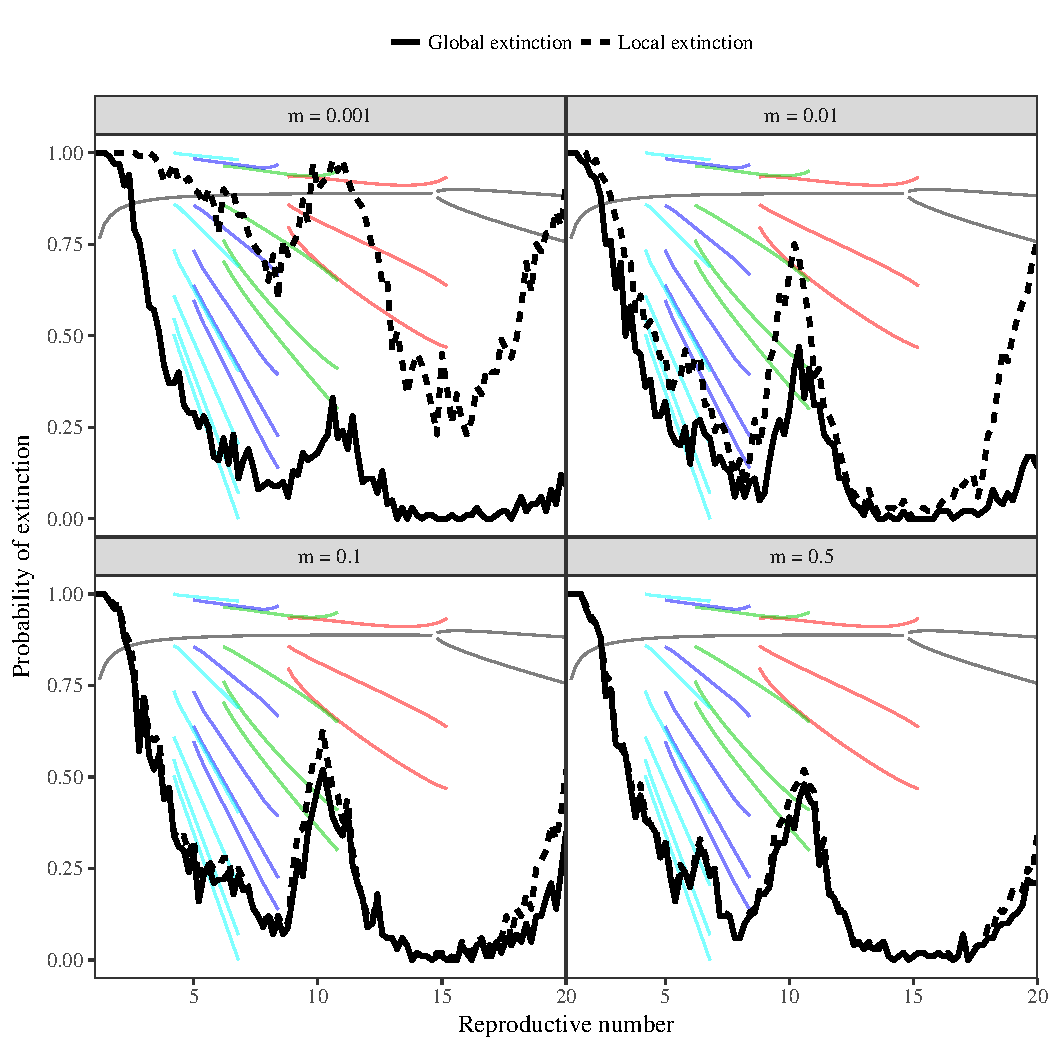
\includegraphics[width=\maxwidth]{figure/unnamed-chunk-7-1} 

\end{knitrout}

\section{Save results for inclusion in main paper}

We now save our figures for use in the final paper.

The plot for probability of coherence:
\begin{knitrout}
\definecolor{shadecolor}{rgb}{0.969, 0.969, 0.969}\color{fgcolor}\begin{kframe}
\begin{alltt}
\hlkwd{ggsave}\hlstd{(}\hlstr{"probabilitycoherence.pdf"}\hlstd{,} \hlkwc{device}\hlstd{=} \hlstr{"pdf"}\hlstd{, gprob.main,} \hlkwc{width}\hlstd{=}\hlnum{7}\hlstd{,} \hlkwc{height} \hlstd{=} \hlnum{5}\hlstd{)}
\end{alltt}
\end{kframe}
\end{knitrout}

\section{Time to generate this document}



CPU time to generate this document: 7.435S seconds

\end{document}
